%%%%%%%%%%%%%%%%%%%%%%%%%%%%%%%%%%%%%%%%%
% FRI Data Science_report LaTeX Template
% Version 1.0 (28/1/2020)
% 
% Jure Demšar (jure.demsar@fri.uni-lj.si)
%
% Based on MicromouseSymp article template by:
% Mathias Legrand (legrand.mathias@gmail.com) 
% With extensive modifications by:
% Antonio Valente (antonio.luis.valente@gmail.com)
%
% License:
% CC BY-NC-SA 3.0 (http://creativecommons.org/licenses/by-nc-sa/3.0/)
%
%%%%%%%%%%%%%%%%%%%%%%%%%%%%%%%%%%%%%%%%%


%----------------------------------------------------------------------------------------
%	PACKAGES AND OTHER DOCUMENT CONFIGURATIONS
%----------------------------------------------------------------------------------------
\documentclass[fleqn,moreauthors,10pt]{ds_report}
\usepackage[english]{babel}
\usepackage{listings}
\usepackage{natbib}
\usepackage{acro}
\graphicspath{{fig/}}
\usepackage{xcolor}
\usepackage{tcolorbox}
\usepackage{subcaption}
\usepackage{cleveref}

\newcommand{\red}[1]{\textcolor{red}{#1}}
\newcommand{\green}[1]{\textcolor{green}{#1}}

\lstset{
frame=none,
}

%----------------------------------------------------------------------------------------
%	ARTICLE INFORMATION
%----------------------------------------------------------------------------------------

% Header
\JournalInfo{FRI Natural language processing course 2025}

% Interim or final report
\Archive{Project report} 
%\Archive{Final report} 

% Article title
\PaperTitle{Conversational Agent with Retrieval-Augmented Generation} 

% Authors (student competitors) and their info
\Authors{Matej Belšak, Gorazd Gorup, Luka Bajić}

% Advisors
\affiliation{\textit{Advisors: Aleš Žagar}}

% Keywords
\Keywords{Conversational agent, Retrieval-Augmented Generation}
\newcommand{\keywordname}{Keywords}


% Abbreviations
\DeclareAcronym{llm}{
	short=LLM,
	long=Large Language Model
}

\DeclareAcronym{rag}{
	short=RAG,
	long=Retrieval Augmented Generation
}

\DeclareAcronym{nlp}{
	short=NLP,
	long=Natural Language Processing
}

\DeclareAcronym{tmdb}{
	short=TMDB,
	long=The Movie Database
}

\DeclareAcronym{fifo}{
	short=FIFO,
	long=First-In-First-Out
}

\newcommand{\etal}{\textit{et al}., }
\newcommand{\ie}{\textit{i}.\textit{e}., }
\newcommand{\eg}{\textit{e}.\textit{g}.\ }

%----------------------------------------------------------------------------------------
%	ABSTRACT
%----------------------------------------------------------------------------------------

\Abstract{
Develop a conversational agent that enhances the quality and accuracy of its responses by dynamically retrieving and integrating relevant external documents from the web. Unlike traditional chatbots that rely solely on pre-trained knowledge, this system will perform real-time information retrieval, ensuring up-to-date answers. Potential applications include customer support, academic research assistance and general knowledge queries. The project will involve natural language processing, web scraping, and retrieval-augmented generation techniques to optimize answer quality.
}

%----------------------------------------------------------------------------------------

\begin{document}

% Makes all text pages the same height
\flushbottom 

% Print the title and abstract box
\maketitle 

% Removes page numbering from the first page
\thispagestyle{empty} 

%----------------------------------------------------------------------------------------
%	ARTICLE CONTENTS
%----------------------------------------------------------------------------------------

\section*{Introduction}
	
While \acp{llm} have evolved considerably and now produce convincing replies, they have inherent limitations. They rely on training data consisting of documents from the past and may not possess knowledge of current events and developments. Due to differences and properties of training datasets, they may not contain specific domain knowledge, failing to answer certain prompts or outright hallucinating. The latter could prove especially disastrous in dedicated chatbots, for example for legal guidance or health care~\cite{thirunavukarasu2023large}.

One possibility would be to retrain the chat model in intervals to try to keep it up to date, but that would still produce periods where the information is missing from the \ac{llm} or is outdated. This approach, while completelly time and energy inefficient, would also not guard against hallucinations. To solve these issues, \ac{rag} is used to provide the missing knowledge to the \ac{llm}. \ac{rag} employs different techniques to retrieve information from external sources based on user’s prompt and through prompt augmentation feed the \ac{llm} sufficient information to provide informative and factually correct answer. In the survey by Gao~\etal~\cite{survey}, multiple approaches to \ac{rag} are presented, highlighting three architectures: naive \ac{rag}, which analyzes the user’s prompt, retrieves the required information and appends it, letting the \ac{llm} do the rest; advanced \ac{rag}, which employs pre-retrieval and post-retrieval modifications to the prompt to make it more suitable for information retrieval and subsequent interpretation by \ac{llm}; lastly, modular \ac{rag} combines multiple approaches, using iterative prompt enhancement, ranking, fusion, etc.

To better evaluate \ac{rag} performance, Lyu~\etal~\cite{benchmark} describe the CRUD framework, employing metrics such as ROUGE, BLEU, precision and recall. Various operations on text (creative generation from context, usage of information to answer questions, identification and correction of false information, summarization, ...) are measured separately to give a more detailed overview of the model. 

For document summarization, \acp{llm}, statistical models, graph-based models and other approaches are used to extract the most important information from text. Zhang~\etal~\cite{summarization} present multiple solutions, noting that \acp{llm}, while consuming more resources, tend to be more coherent and precise in their summarization if trained correctly.

In this paper, we focus on \ac{rag} methods and their use in chatbots. To that end, we design a conversational agent operating on knowledge about different art and media. Specifically, the agent is to suggest and converse about films and other related media based on the user’s prompts and preferences. Our contributions are:

\begin{itemize}
	\item Implementation of a conversational agent using two different pretrained models: DeepSeek-R1~\cite{deepseek3} and Qwen 3~\cite{qwen3}.
	\item Implementation of two \ac{rag} techniques, a primitive and advanced one, with capabilities of retrieving data from various film-related databases and web sources.
	\item Evaluation of conversational agents with respect to the model used and the \ac{rag} technique. Agents are evaluated against the baseline \ac{rag}-less chatbots. Human and \ac{llm} judges are used to score responses, and different metrics are analyzed.
\end{itemize}

%------------------------------------------------

\section*{Methods}

We designed two \ac{rag} pipelines, as presented in~\cref{fig:pipeline}. The naive RAG pipeline used \ac{nlp} methods to extract the important feature information from prompt via lemmatization, stop-word removal, and entity detection. Prompt information was used to determine movie titles and names of people to query for in our selected databases. That information was then appended to the prompt and fed into an \ac{llm}.

A more advanced version of our \ac{rag} system utilized various components, but we ultimately chose to employ function-calling functionality that is present in some \acp{llm}. Based on the prompt, the \ac{llm} decides on the most appropriate information retrieval function to call and informs the \ac{rag} system, which then retrieves that information. The information is then inserted into the prompt, which is fed into the \ac{llm}.

\begin{figure*}
	\centering
	\begin{subfigure}{0.4\textwidth}
		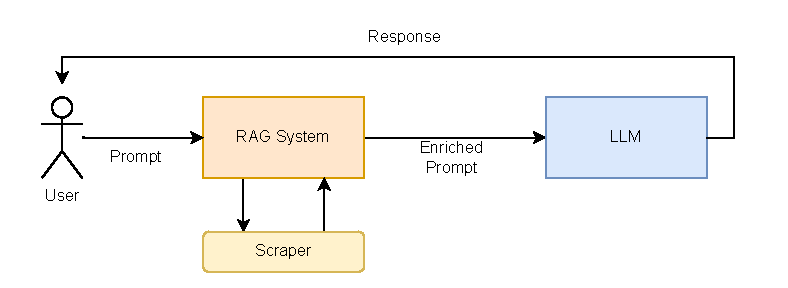
\includegraphics[width=\textwidth]{./figures/simple_rag.pdf}
		\caption{A naive \ac{rag} system.}
	\end{subfigure}
	\hspace{20pt}
	\begin{subfigure}{0.4\textwidth}
		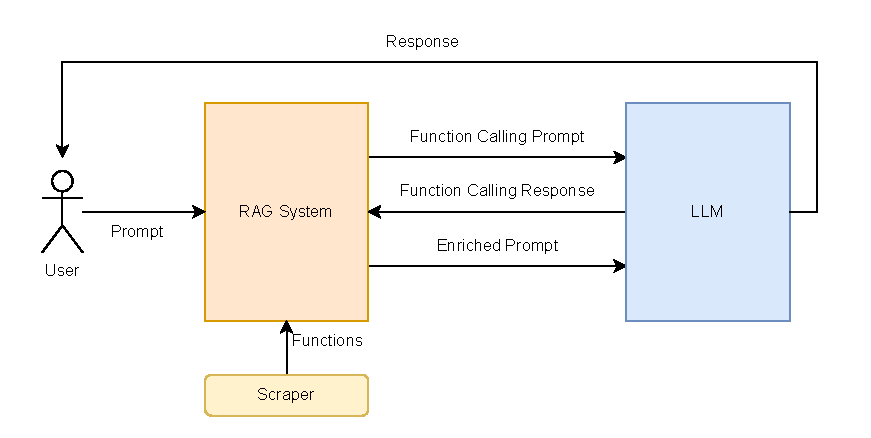
\includegraphics[width=\linewidth]{./figures/advanced_rag.pdf}
		\caption{An advanced \ac{rag} system.}
	\end{subfigure}
	\caption{Our proposed \ac{rag} pipelines for evaluation. The naive \ac{rag} variant preprocesses the prompt, extracts meaningful information from it, retrieves the data based on that, and enhances the prompt with that raw data. The advanced variant employs \ac{llm} function-calling capabilities to decide what data to scrape and enhances the prompt only with necessary data.}
	\label{fig:pipeline}
\end{figure*}

\subsection*{Models}

To better analyze the impact and viability of \ac{rag} on different \acp{llm}, we decided to use two models: one with reasoning capabilities and one without.

Since we were limited by hardware capabilities during our research, we focused on models with quantizied or distilled variants. We ultimatelly decided on a Qwen3~\footnote{https://huggingface.co/Qwen/Qwen3-8B} model as our non-reasoning \ac{llm}, and a distilled Llama variant of DeepSeek R1~\footnote{https://huggingface.co/deepseek-ai/DeepSeek-R1} as our reasoning \ac{llm}. Both models were 8-billion-parameters versions. We chose DeepSeek as it is a novel set of models with positive benchmarking results~\cite{deepseek3}.

Both models were loaded from HuggingFace and were run through the \texttt{transformers} API.

\subsubsection*{Function Calling}

In some cases, we leveraged the function calling capabilities of our models. While DeepSeek hints at possibility of using this feature~\cite{deepseekFunctionCalling}, their proposed prompt templates do not support it. We instead turned to Qwen's function calling capabilities, which proved to be sufficient.

In function calling, the model is presented with the user prompt and structured information about programmatic functions it may call to fullfil the user's request. The \ac{llm} is tought to return a similarly structured set of instructions on which functions to call, and with what parameters.

\subsection*{Information Retrieval}

To provide a sufficient level of information related to movies and similar media, we selected the following sources:

\begin{itemize}
	\item \textbf{\ac{tmdb}.} This is an open database of movies, TV-shows, and people associated with them. They provide a free-to-use API for various types of requests -- release dates, cast, crew, similar films ...
	\item \textbf{Letterboxd.} This is a movie-themed social network to log watched films, provide reviews, and engage in movie-related discussions. We chose to include it to give the model a better understanding of how people percieve certain media.
	\item \textbf{JustWatch.} This website tracks the availability of media on digital and streaming platforms.
	\item \textbf{Wikipedia.} We used it to retrieve information such as film plots, summaries, etc.
\end{itemize}

In our naive \ac{rag} implementation, we retrieved data from all four sources. This would amount to over 250,000 characters of context.

For our advanced version, we prepared nine custom scraping functions that would equip the model with essential information about movie titles and film-related people. These functions had to be specifically annotated and various versions of descriptions were used to elicit a proper function-calling response from the model.

\subsection*{\ac{rag}}

For the naive \ac{rag} system, we first analyzed the user prompt and gathered all relevant entities, consisting of film titles and names of people. We used a Roberta-like \texttt{spacy} model~\footnote{https://huggingface.co/spacy/en\_core\_web\_sm}. We performed unfiltered knowledge injection, gathering all relevant documents based on prompt entities, structured them in JSON format, and passed them allong with user query to the \ac{llm}.

For advanced \ac{rag} system, we tried several versions before basing it on function calling. Our earlier attempts performed the entity extraction from prompt, retrieval of documents from all sources based on those entities, and content curation based on statistical methods and user prompt. For example, we treated all sentences in the retrieved data as documents, performing TF-IDF sorting and using only top $N$ most relevant sentences. Unfortunatelly, results of these extractions accounted only for literal appearance of words from the prompt in documents, instead of accounting for larger context, synonyms, etc.

To address these shortcomings, we turned to function calling, letting the \ac{llm} decide what information to retrieve. In the system prompt, we also appended additional information about current date for better context formulation.

\subsection*{Prompt formulation}

We structured our prompts to consist of three roles: system, user, and assistant. We put system prompt first, followed by the user prompt, and finally by assistant tag to signal the \ac{llm} to generate the answer, not to continue the user prompt.

Our system prompt was:

\begin{figure}[h!]
	\begin{tcolorbox}
		You are an AI chatbot, assisting user with anything related to movies. [Today's date is \verb|{date}|.] You may only use information provided to you inside the \verb|<data>| tags.
	\end{tcolorbox}
	\caption{Out prompt for \ac{rag} usage. The text in square brackets was only used in advanced \ac{rag}, and the text in braces represents variables.}
\end{figure}

Our user prompt first presented the user's initial query, followed by the retrieved information enclosed in \verb|<data>| tags.

\subsection*{Memory}

Because we designed our agent as a chatbot, we also implemented a simple answer caching mechanism to provide the chatbot with immediate history of the conversation. We stored last $n$ user questions and chatbot replies with the \ac{fifo} method, and fed them to the \ac{llm} as part of the prompt. The $n$ in our observations had to be relatively small due to limitations on the amount of input tokens.

% In advanced \ac{rag}, we observed that the memory mechanism prevented the chatbot from being confused about queries referencing previous ones, managing to remember crucial data for function calling. Sometimes, the \ac{llm} even decided against retrieving information in queries where it otherwise would, because previous questions and answers provided enough information or context to formulate a sufficient response.


\subsection*{Evaluation methodology}

Since we are working with relatively open-ended questions, there is a lack of objective ground truth to evaluate against. Therefore, we construct a set of 50 domain-relevant questions and use manually checked answers from the commercial ChatGPT model as ground truth for metric computations. To avoid overfitting a model to a specific set of expected outputs, we included multiple types of questions into our test set, including yes/no questions, fact checking, list retrieval and summarization. All queries are zero-shot.


\subsubsection*{LLM-based evaluation}

Standard evaluation metrics such as BLEU and ROUGE are ill-adjusted to our test set, because they penalize diverse answers, which could still be correct in the context of open-ended questions. To bypass this limitation, we employ the DeepEval framework \cite{deepeval} in order to obtain more relevant metrics based on context, query and response:

\begin{itemize}
	\item correctness: compares similarity of the response with the ground truth,
	\item clarity: measures readability of the text (we do not expect to improve this metric with \ac{rag}, we only utilize it to ensure that our modifications do not degrade the original model's inherent capabilities),
	\item answer relevancy: determines to which extent the response is related to the query,
	\item faithfulness: determines to which extent the retrieved documents are represented in the response,
	\item contextual precision: measures the correctness of retrieved documents.
	\item contextual recall: measures the completeness of retrieved documents.
	\item contextual relevancy: measures the relevance of retrieved documents.
\end{itemize} 



\section*{Results}

\begin{table*}[t]
%\centering
\resizebox{1.0 \linewidth}{!}{\begin{tabular}{| r | c c c c c c c |}
\hline
model & correctness & clarity & answer relevancy & faithfulness & contextual precision & contextual recall & contextual relevancy \\ \hline
deepseek-baseline  & 0.19 & 0.7725 & 0.76846 & / & / & / & / \\
deepseek-naive  & 0.152 & 0.82800 & 0.78138 & 0.93233 & 0.24000 & 0.61771 & \textbf{0.40468}   \\
deepseek-advanced  & & & & & & &   \\
qwen-baseline  & \textbf{0.30962} & \textbf{0.86888} & 0.74805 & / & / & / & /  \\
qwen-naive  & 0.23111 & 0.65888 & \textbf{0.84670} & 0.88345 & \textbf{0.88345} & \textbf{0.76333} & 0.37029  \\
qwen-advanced  &  & & &  &  & &    \\
\hline
\end{tabular}}
\caption{Performance comparison as evaluated by a 14B-parameter Qwen model with DeepEval framework.}
\label{tab:llm_metrics}
\end{table*}

\begin{table*}[t]
%\centering
\resizebox{1.0 \linewidth}{!}{\begin{tabular}{| r | c c c c c c c |}
\hline
model & correctness & clarity & answer relevancy & faithfulness & contextual precision & contextual recall & contextual relevancy \\ \hline
deepseek-baseline  & 0.31845 & 0.74923 & 0.61720 & / & / & / & / \\
deepseek-naive  & 0.33410 & 0.81443 & 0.720714 & 0.75611 & 0.34 & 0.32014 & 0.43623   \\
deepseek-advanced & 0.33412 & 0.78414 & 0.80973 & 0.93095 & \textbf{1.0} & 0.60937 & 0.56813   \\
qwen-baseline  & 0.45205 & 0.81023 & \textbf{0.87944} & / & / & / & /  \\
qwen-naive  & 0.45116 & 0.77992 & 0.80013 & 0.83234 & 0.34 & 0.264401 & 0.51643  \\
qwen-advanced  & \textbf{0.52336} & \textbf{0.83382} & 0.68042 & \textbf{0.97935} & \textbf{1.0} & \textbf{0.61096} & \textbf{0.68355}   \\
\hline
\end{tabular}}
\caption{Performance comparison as evaluated by GPT-4.1-mini model with DeepEval framework.}
\label{tab:gpt}
\end{table*}

In this section we compare the performance of a reasoning DeepSeek-R1-Distill-Llama-8B \cite{deepseek3} model and a non-reasoning Qwen3-8B \cite{qwen3} model. For each of these we run experiments on three different sets of parameters:
\begin{itemize}
	\item without \ac{rag} - out-of-the-box model with no modifications (baseline)
	\item with naive \ac{rag} - all documents are retrieved and appended to the context with no consideration for token limitation (data is truncated)
	\item advanced \ac{rag} - documents are selectively retrieved and processed before being appended to the context
\end{itemize}

Results obtained with Qwen-14B model are shown in Table \ref{tab:llm_metrics}. Metrics related to context are not available for baseline models, because their context is an empty set. Models with advanced \ac{rag} can choose not to retrieve documents, depending on the question, so the metrics are only computed when at least one document was retrieved. 

Because the model used for evaluation is not drastically larger than the model used for response generation, it is sensible to repeat the same experiments with an even larger LLM to obtain more reliable results. We opted for GPT-4.1-mini. Results are shown in Table \ref{tab:gpt}. Due to computational complexity, we compute the metrics on first 25 questions in the test set and report the average values. 



\subsection*{Conversational chatbot}

Extending a question answering model into a conversational chatbot is straightforward: the information retrieval pipeline remains the same, we only need to implement a mechanism for memorization of previous questions and responses. Examples of Qwen chatbot results are shown in Appendix \ref{qwenconvo}.


%------------------------------------------------

\section*{Discussion}

We conclude that it is possible to improve the responses of 8B-parameter LLMs, such as Qwen and DeepSeek on queries from a specific domain by employing on-the-fly information retrieval via web scraping. 

Superior performance is achieved by constructing document retrieval functions in such a way that an LLM can be used not only to generate a response, but also to determine which documents are relevant based on the user query. 

A question answering model with \ac{rag} can be extended into a chatbot by implementing a memory mechanism, which stores a buffer of previous questions, which allows the model to keep track of recent conversation.



%----------------------------------------------------------------------------------------
%	REFERENCE LIST
%----------------------------------------------------------------------------------------
\bibliographystyle{unsrt}
\bibliography{report}

\newpage
\begin{appendix}

\section*{Appendix}
\label{append}

\subsection*{Qwen conversation example}

\begin{figure}
\begin{tcolorbox}
User: How many films did Chuck Jones make?

Qwen: Based on the data provided:

	**Total Number of Films:**  
	Chuck Jones directed **over 100 films**, spanning multiple genres and formats.

	\#\#\# Breakdown:
	- **Feature-Length Films**: 
    		- *The Bugs Bunny/Road Runner Movie* (1979)
	    - *The Phantom Tollbooth* (1970)
	    - *The Grinch Stole Christmas!* (1966)

	- **Shorts and Documentaries**:
	    - Approximately **100+ short cartoons**
	        - Many of these are Looney Tunes/Merry Melodies cartoons.
	        - Includes iconic titles such as *What's Opera, Doc?*, *Duck Amuck*, etc.
    
	    - **Documentaries**: Around **dozens**, e.g.,
	    	    - *The Magical World of Chuck Jones*
	        - *Chuck Jones: Memories of Childhood*

	\#\#\# Summary:
	Chuck Jones made approximately \textbf{more than 100 films}, primarily consisting of **\green{animated short cartoons}**, a handful of **\green{feature-length compilations}**, and several **\red{documentaries}**.
\end{tcolorbox}
\caption{Conversation with Qwen}
\label{qwenconvo}
\end{figure}

\begin{figure*}
\begin{tcolorbox}
\begin{lstlisting}[escapechar=\%]Add commentMore actions
User: How many films did Chuck Jones make?

Qwen: Based on the data provided:

	**Total Number of Films:**  
	Chuck Jones directed **over 100 films**, spanning multiple genres and formats.

	### Breakdown:
	- **Feature-Length Films**: 
    		- *The Bugs Bunny/Road Runner Movie* (1979)
	    - *The Phantom Tollbooth* (1970)
	    - *The Grinch Stole Christmas!* (1966)

	- **Shorts and Documentaries**:
	    - Approximately **100+ short cartoons**
	        - Many of these are Looney Tunes/Merry Melodies cartoons.
	        - Includes iconic titles such as *What's Opera, Doc?*, *Duck Amuck*, etc.

	    - **Documentaries**: Around **dozens**, e.g.,
	    	    - *The Magical World of Chuck Jones*
	        - *Chuck Jones: Memories of Childhood*


	Chuck Jones made approximately **more than 100 films**, primarily consisting of **%\green{animated short cartoons}%**, a handful of **%\green{feature-length compilations}%**, and several **%\red{documentaries}%**.
\end{lstlisting}
\end{tcolorbox}
\caption{Conversation with Qwen}
\label{qwenconvo}
\end{figure*}


 


\end{appendix}


\end{document}